\section{Proposed Method: \diffgnn}
\label{sec:method}
Building on the relaxed formulation in Section~\ref{sec:preliminaries}, we propose \diffgnn, a differentiable graph neural framework for jointly optimizing HW/SW partitioning and scheduling. Rather than directly searching over discrete assignments $\vx \in \{0,1\}^n$, \diffgnn learns a continuous hardware assignment vector $\vp \in [0,1]^n$ together with software ordering scores $\vq^{sw}$, and optimizes the relaxed objective in Equation~\ref{eq:relaxed_objective} end-to-end using gradient-based learning.

Figure~\ref{fig:diff_gnn_architecture} illustrates the overall pipeline.
Given a task graph $\gG(\gV, \gE)$, we first prepare the node features $\mF$, and a GNN encoder computes node embeddings, which are then consumed by two prediction heads.
(i) a \emph{placement head} that predicts relaxed hardware assignment probabilities, and (ii) an \emph{ordering head} that predicts software scheduling priorities. 
These outputs are passed to an order-aware differentiable scheduler that approximates the makespan while accounting for both precedence constraints and software serialization. During inference, the relaxed solution is discretized, repaired if necessary to satisfy the area constraint, optionally refined, and finally evaluated using list scheduling with static priorities (LSSP).

\begin{figure*}[t]
\centering
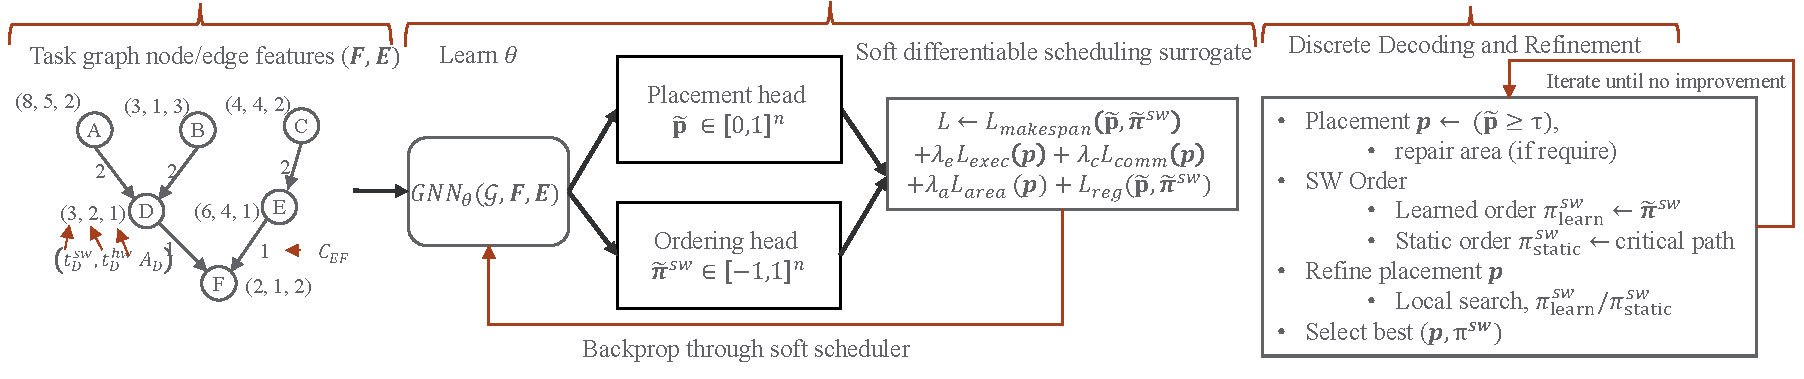
\includegraphics[width=1.0\linewidth]{Figures/methods/GNN_placement_order.pdf}
\caption{\sid{placeholder} Overview of \texttt{Diff-GNN} for joint HW/SW partitioning and scheduling. A GNN encoder maps task graph features to soft placement probabilities $\mathbf{p}$ and scheduling priorities $\mathbf{q}^{sw}$. A differentiable scheduling surrogate enables end-to-end optimization of makespan under constraints. At inference, solutions are discretized, repaired for feasibility, optionally refined (DLS/LSSP), and evaluated via list scheduling to obtain the final makespan.}
\label{fig:diff_gnn_architecture}
\end{figure*}


\subsection{Input Feature Preparation}

\paragraph{\textbf{Node features.}}
Each node $i \in \gV$ is associated with a feature vector capturing execution cost, resource usage, and structural properties:
\begin{equation}
\vf_i^{\mathrm{raw}} =
\left[
t_i^{sw},\;
t_i^{hw},\;
A_i,\;
d_i,\;
\frac{t_i^{hw}}{t_i^{sw}+\epsilon},\;
t_i^{sw}-t_i^{hw},\;
\frac{t_i^{sw}-t_i^{hw}}{\max(A_i,\epsilon)}
\right]
\in \mathbb{R}^7.
\end{equation}

Stacking all node features yields the feature matrix
\begin{equation}
\mF^{\mathrm{raw}} =
\begin{bmatrix}
(\vf_1^{\mathrm{raw}})^\top\\
\vdots\\
(\vf_n^{\mathrm{raw}})^\top
\end{bmatrix}
\in \mathbb{R}^{n \times 7}.
\end{equation}

We normalize features across nodes using column-wise z-score normalization:
\begin{equation}
\tilde{\mF} = \mathrm{Norm}(\mF^{\mathrm{raw}}).
\end{equation}

To incorporate the global hardware-area constraint, we append a constant feature:
\begin{equation}
\mF =
\begin{bmatrix}
\tilde{\mF} & \rho_A \mathbf{1}
\end{bmatrix}
\in \mathbb{R}^{n \times 8},
\end{equation}
where $\mathbf{1}\in\mathbb{R}^{n}$ is the all-ones vector.

\paragraph{\textbf{Edge features.}}
For each directed edge $(i,j) \in \gE$, we define an edge feature vector:
\begin{equation}
\ve_{ij}^{\mathrm{raw}} =
\left[
C_{ij},\;
|g_i - g_j|,\;
|ga_i - ga_j|
\right]
\in \mathbb{R}_{\ge 0}^3.
\end{equation}

Stacking all edges yields the edge-feature matrix
\begin{equation}
\mE^{\mathrm{raw}} \in \mathbb{R}^{|\gE| \times 3}.
\end{equation}

We normalize edge features using column-wise max scaling:
\begin{equation}
\mE = \mathrm{Norm}_\infty(\mE^{\mathrm{raw}}),
\end{equation}
where $\mathrm{Norm}_\infty(\cdot)$ denotes feature-wise normalization by the maximum value.


\subsection{GNN Module}

\paragraph{\textbf{Message passing.}}
Let $\vh_i^{(0)} = \mF_{i,:}$ denote the initial node embedding. We use a message-passing GNN with $L$ layers:
\begin{equation}
\vh_i^{(\ell+1)} =
\phi^{(\ell)}\!\left(
\vh_i^{(\ell)},
\operatorname*{AGG}_{j:(j,i)\in\gE}
\psi^{(\ell)}\!\left(
\vh_i^{(\ell)},\;
\vh_j^{(\ell)},\;
\ve_{ji}
\right)
\right),
\end{equation}
for $\ell = 0,\dots,L-1$, where $\phi^{(\ell)}$ and $\psi^{(\ell)}$ are learnable functions and $\operatorname*{AGG}$ is a permutation-invariant aggregation operator.
As a concrete instantiation, we use weighted mean aggregation:
\begin{align*}
\operatorname*{AGG}_{j:(j,i)\in\gE}
\psi^{(\ell)}\!\left(
\vh_i^{(\ell)},\;
\vh_j^{(\ell)},\;
\ve_{ji}
\right)
=\\
\frac{1}{\sum_{j\in\gN(i)} \alpha_{\phi}(j,i) + \epsilon}
\sum_{j\in\gN(i)}
\alpha_{\phi}(j,i)\,\mathbf{W}^{(\ell)}\vh_j^{(\ell)},
\end{align*}
where $\gN(i)$ denotes the set of incoming neighbors of node $i$, $\mathbf{W}^{(\ell)}$ is a learnable linear transformation, and $\alpha_{\phi}(j,i)\ge 0$ is a learnable edge weight from $\ve_{ji}$.
We compute edge weights directly from edge features:
\begin{equation}
\alpha_{\phi}(j,i) = \sigma\!\left(f_{\phi}(\ve_{ji})\right),
\end{equation}
where $f_{\phi}$ is an MLP and $\sigma(\cdot)$ is the sigmoid function, ensuring $\alpha_{\phi}(j,i)\in(0,1)$.

\paragraph{\textbf{Placement head.}}
From the final embedding $\vh_i^{(L)}$, we directly predict hardware-assignment probabilities:
\begin{equation}
p_i = \sigma\!\left(\mathrm{MLP}_{\mathrm{place}}(\vh_i^{(L)})\right),
\end{equation}
where $\sigma(\cdot)$ denotes the sigmoid function, ensuring $p_i \in (0,1)$.

The vector $\vp = [p_1,\dots,p_n]^\top$ represents the relaxed placement probabilities.

\paragraph{\textbf{Ordering head.}}
To model software execution order, we compute bounded ordering scores:
\begin{equation}
q_i^{sw} = \tanh\!\left(\mathrm{MLP}_{\mathrm{order}}(\vh_i^{(L)})\right),
\end{equation}
so that $q_i^{sw} \in (-1,1)$ and stacking all scores yields $\vq^{sw} \in \mathbb{R}^n$.



\subsection{Differentiable Soft Scheduler}

We now instantiate the relaxed makespan term $\widetilde{\mathrm{Makespan}}(\vp,\vq^{sw})$ from Section~\ref{sec:preliminaries}. The scheduler takes as input the relaxed placement vector $\vp$ and the software ordering scores $\vq^{sw}$, and produces approximate start and finish times for all tasks.

\paragraph{\textbf{From ordering scores to soft pairwise precedence.}}
The ordering head outputs software-priority scores
\begin{equation}
\vq^{sw} = [q_1^{sw},\ldots,q_n^{sw}]^\top.
\end{equation}
Since the final software execution order is a permutation, we first map these scores to a soft permutation matrix using a differentiable sorting relaxation. Specifically, we construct a score-to-position compatibility matrix
\begin{equation}
L_{ai} = -\frac{(q_i^{sw}-u_a)^2}{\tau_o},
\qquad
u_a = 1-\frac{2a}{n-1},
\quad a=0,\ldots,n-1,
\end{equation}
where $\{u_a\}_{a=0}^{n-1}$ are evenly spaced position anchors and $\tau_o$ controls the sharpness of the relaxation. Applying Sinkhorn normalization gives
\begin{equation}
\mP^{sw} = \mathrm{Sinkhorn}(L) \in [0,1]^{n\times n},
\end{equation}
where $\mP^{sw}_{ai}$ is the soft probability that task $i$ occupies position $a$ in the software execution order.
Next we compute the expected soft rank of each task:
\begin{equation}
\tilde r_i = \sum_{a=0}^{n-1} a\,P^{sw}_{ai}.
\end{equation}
We then define pairwise precedence using a sigmoid over rank differences:
\begin{equation}
B^{sw}_{ji}
=
\sigma\!\left(\frac{\tilde r_i-\tilde r_j}{\tau_r}\right),
\qquad
B^{sw}_{ii}=0,
\end{equation}
where $\tau_r$ controls the sharpness of the pairwise comparison. Thus, $B^{sw}_{ji}$ is large when task $j$ is likely to precede task $i$.

Since ordering matters only when both tasks are assigned to software, we gate the pairwise precedence by the soft software co-assignment:
\begin{equation}
R^{sw}_{ji}=B^{sw}_{ji}(1-p_j)(1-p_i).
\end{equation}

We do not predict ranks directly from GNN because ranks are discrete and depend on sorting, which is not differentiable. Likewise, directly converting raw ordering scores into pairwise probabilities using only score differences, e.g.,
\(
\sigma((q_i^{sw}-q_j^{sw})/\tau),
\)
does not enforce a globally consistent permutation structure. Such pairwise comparisons may violate transitivity and need not correspond to any valid total order. The Sinkhorn relaxation addresses this issue by first constructing an approximately doubly stochastic matrix, which serves as a continuous surrogate of a permutation matrix. The rank-sigmoid form then provides a more efficient way to derive pairwise precedence from this structured relaxation.

\paragraph{\textbf{Step 1: relaxed execution and communication.}}
The relaxed execution time of node $i$ is
\begin{equation}
\tilde{t}_i(\vp)=p_i t_i^{hw} + (1-p_i)t_i^{sw},
\end{equation}
and the relaxed communication delay on edge $(j,i)$ is
\begin{equation}
\tilde{c}_{ji}(\vp)=|p_j-p_i|\,C_{ji}.
\end{equation}

\paragraph{\textbf{Step 2: DAG readiness.}}
Let $\Pred(i)$ denote the set of predecessors of node $i$. The DAG-readiness term captures when all dependency constraints are satisfied:
\begin{equation}
r_i^{dag}
=
\begin{cases}
0, & \Pred(i)=\emptyset,\\[4pt]
\mathrm{LSE}_{\beta}
\Big(
\{\, f_j + \tilde{c}_{ji}(\vp) \mid j \in \Pred(i)\,\}
\Big), & \text{otherwise},
\end{cases}
\end{equation}
where
\begin{equation}
\mathrm{LSE}_{\beta}(\{a_k\}) = \frac{1}{\beta}\log\sum_k e^{\beta a_k}.
\end{equation}
Intuitively, $r_i^{dag}$ is the earliest soft time at which node $i$ becomes ready from the precedence perspective.

\paragraph{\textbf{Step 3: resource readiness.}}
Because software tasks execute sequentially on a single CPU, node $i$ may also need to wait for other software tasks predicted to execute before it. We therefore define the software resource-readiness term as
\begin{equation}
r_i^{sw}
=
\mathrm{LSE}_{\beta}
\Big(
\{\, f_j + \alpha \log(R^{sw}_{ji}+\epsilon) \mid j \neq i\,\}
\Big),
\end{equation}
where $\alpha$ controls the influence of the soft ordering gate and $\epsilon$ is a small constant for numerical stability. If $R^{sw}_{ji}$ is large, then task $j$ is likely to precede task $i$ on software, and its finish time contributes strongly to the readiness of $i$.

\paragraph{\textbf{Step 4: start and finish times.}}
The soft start time of node $i$ is obtained by combining the DAG and resource readiness terms:
\begin{equation}
s_i = \mathrm{LSE}_{\beta}\big(\{r_i^{dag},\, r_i^{sw}\}\big).
\end{equation}
The corresponding soft finish time is
\begin{equation}
f_i = s_i + \tilde{t}_i(\vp).
\end{equation}

\paragraph{\textbf{Step 5: soft makespan.}}
Let $\Sink(\gG)$ denote the set of sink nodes in $\gG$. The relaxed makespan is then
\begin{equation}
L_{\mathrm{soft\mbox{-}makespan}}(\vp,\vq^{sw})
=
\widetilde{\mathrm{Makespan}}(\vp,\vq^{sw})
=
\mathrm{LSE}_{\beta}\big(\{\, f_i \mid i \in \Sink(\gG)\,\}\big).
\end{equation}

Overall, the scheduler combines two timing signals: (i) DAG readiness, which captures dependency completion, and (ii) resource readiness, which captures serialization on the software processor. This coupling allows \diffgnn to optimize placement and ordering jointly.

\paragraph{\textbf{Illustrative 6-node example.}}
Let us consider the task graph in Figure~\ref{fig:demosoftmakespanI}. For this example, the placement head predicts
\begin{equation}
\vp=[0.05,\,0.05,\,0.05,\,0.95,\,0.95,\,0.95]^\top,
\end{equation}
for tasks $(A,B,C,D,E,F)$, indicating that $A,B,C$ are likely assigned to software, while $D,E,F$ are likely assigned to hardware. The ordering head predicts
\begin{equation}
\vq^{sw}=[0.00,\,-1.00,\,1.00,\,-0.50,\,-0.75,\,-0.25]^\top,
\end{equation}
which induces the preference \(C \prec A \prec B\) among the software tasks.

Under our soft-makespan formulation, the order \(C \prec A \prec B\) yields a smaller makespan than \(A \prec B \prec C\). The reason is that once task $C$ finishes, task $E$ can start on hardware in parallel with the subsequent execution of $A$ and $B$ on software. As a result, by the time tasks $A$ and $B$ complete and task $D$ finishes, task $E$ is already close to completion or finished, allowing task $F$ to start earlier. In contrast, if the order is \(A \prec B \prec C\), the $C \rightarrow E$ branch is delayed and the overall makespan increases.

Without the ordering head, a scheduler based only on DAG readiness cannot distinguish among the ready source tasks $A$, $B$, and $C$, since all of them are valid starting points under the precedence constraints. Consequently, this schedule-sensitive distinction is not captured. A detailed step-by-step illustration is provided in Appendix~\ref{app:illustration}.

\begin{figure}[!htbp]
\centering
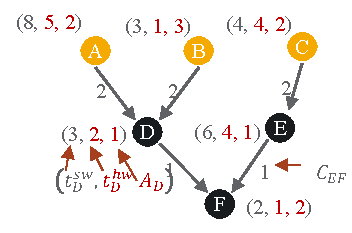
\includegraphics[width=0.52\linewidth]{Figures/methods/demosoftmakespan.pdf}
\caption{Illustrative 6-node fork-join task graph used to explain the differentiable soft scheduler. Each node is annotated with $(t_i^{sw}, t_i^{hw}, A_i)$, and each edge label denotes communication cost.}
\label{fig:demosoftmakespanI}
\end{figure}

\subsection{Differentiable Soft Scheduler}

We now instantiate the relaxed makespan term $\widetilde{M}(\tilde{\vp},\tilde{\vpi}^{sw})$ from Section~\ref{sec:preliminaries}. The scheduler takes as input the relaxed placement vector $\tilde{\vp}$ and the relaxed software-priority vector $\tilde{\vpi}^{sw}$, and produces approximate start and finish times for all tasks.

\paragraph{\textbf{From relaxed software priorities to soft pairwise precedence.}}
The ordering head outputs
\begin{equation}
\tilde{\vpi}^{sw}=[\tilde{\pi}_1^{sw},\ldots,\tilde{\pi}_n^{sw}]^\top.
\end{equation}
Since the final software execution order is a permutation, we first map these values to a soft permutation matrix using a differentiable sorting relaxation. Specifically, we construct a score-to-position compatibility matrix
\begin{equation}
L_{ai}=-\frac{(\tilde{\pi}_i^{sw}-u_a)^2}{\tau_o},
\qquad
u_a=1-\frac{2a}{n-1},
\quad a=0,\ldots,n-1,
\end{equation}
where $\{u_a\}_{a=0}^{n-1}$ are evenly spaced position anchors and $\tau_o$ controls the sharpness of the relaxation. Applying Sinkhorn normalization gives
\begin{equation}
\mP^{sw} = \mathrm{Sinkhorn}(L)\in[0,1]^{n\times n},
\end{equation}
where $\mP^{sw}_{ai}$ is the soft probability that task $i$ occupies position $a$ in the software execution order.

Next we compute the expected soft rank of each task:
\begin{equation}
\tilde{r}_i = \sum_{a=0}^{n-1} a\, \mP^{sw}_{ai}.
\end{equation}
We then define pairwise precedence using a sigmoid over rank differences:
\begin{equation}
B^{sw}_{ji}
=
\sigma\!\left(\frac{\tilde{r}_i-\tilde{r}_j}{\tau_r}\right),
\qquad
B^{sw}_{ii}=0,
\end{equation}
where $\tau_r$ controls the sharpness of the pairwise comparison. Thus, $B^{sw}_{ji}$ is large when task $j$ is likely to precede task $i$.

Since ordering matters only when both tasks are assigned to software, we gate the pairwise precedence by the soft software co-assignment:
\begin{equation}
R^{sw}_{ji}=B^{sw}_{ji}(1-\tilde{p}_j)(1-\tilde{p}_i).
\end{equation}

The Sinkhorn relaxation is used because directly predicting discrete ranks is not differentiable, and directly converting relaxed software-priority values to pairwise probabilities using only score differences does not guarantee a globally consistent order.

\paragraph{\textbf{Step 1: relaxed execution and communication.}}
The relaxed execution time of node $i$ is
\begin{equation}
\tilde{t}_i(\tilde{\vp})=\tilde{p}_i t_i^{hw} + (1-\tilde{p}_i)t_i^{sw},
\end{equation}
and the relaxed communication delay on edge $(j,i)$ is
\begin{equation}
\tilde{c}_{ji}(\tilde{\vp})=|\tilde{p}_j-\tilde{p}_i|\,C_{ji}.
\end{equation}

\paragraph{\textbf{Step 2: DAG readiness.}}
Let $\Pred(i)$ denote the set of predecessors of node $i$. The DAG-readiness term captures when all dependency constraints are satisfied:
\begin{equation}
s_i^{dag}
=
\begin{cases}
0, & \Pred(i)=\emptyset,\\[4pt]
\mathrm{SMax}_{\beta}
\Big(
\{\, \tilde{f}_j + \tilde{c}_{ji}(\tilde{\vp}) \mid j \in \Pred(i)\,\}
\Big), & \text{otherwise},
\end{cases}
\end{equation}
where
\begin{equation}
\mathrm{SMax}_{\beta}(\{a_k\}) = \frac{1}{\beta}\log\sum_k e^{\beta a_k}.
\end{equation}
Intuitively, $s_i^{dag}$ is the earliest soft time at which node $i$ becomes ready from the precedence perspective.

\paragraph{\textbf{Step 3: software readiness.}}
Because software tasks execute sequentially on a single CPU, node $i$ may also need to wait for other software tasks predicted to execute before it. Consistent with the relaxed software-serialization term in Section~\ref{sec:preliminaries}, we define
\begin{equation}
\phi_{sw}(\tilde{\pi}_j^{sw},\tilde{\pi}_i^{sw})
=
\alpha \log(R^{sw}_{ji}+\epsilon),
\end{equation}
and the software-readiness term as
\begin{equation}
s_i^{sw}
=
\mathrm{SMax}_{\beta}
\Big(
\{\, \tilde{f}_j + \phi_{sw}(\tilde{\pi}_j^{sw},\tilde{\pi}_i^{sw}) \mid j \neq i\,\}
\Big).
\end{equation}
Here, $\alpha$ controls the influence of the relaxed software order and $\epsilon$ is a small constant for numerical stability. If $R^{sw}_{ji}$ is large, then task $j$ is likely to precede task $i$ on software, and its finish time contributes more strongly to the readiness of $i$.

\paragraph{\textbf{Step 4: start and finish times.}}
The relaxed start time of node $i$ is obtained by combining the DAG and software-readiness terms:
\begin{equation}
\tilde{s}_i = \mathrm{SMax}_{\beta}\big(\{s_i^{dag},\, s_i^{sw}\}\big).
\end{equation}
The corresponding relaxed finish time is
\begin{equation}
\tilde{f}_i = \tilde{s}_i + \tilde{t}_i(\tilde{\vp}).
\end{equation}

\paragraph{\textbf{Step 5: soft makespan.}}
Let $\Sink(\gG)$ denote the set of sink nodes in $\gG$. The relaxed makespan is then
\begin{equation}
L_{\mathrm{soft\mbox{-}makespan}}(\tilde{\vp},\tilde{\vpi}^{sw})
=
\widetilde{M}(\tilde{\vp},\tilde{\vpi}^{sw})
=
\mathrm{SMax}_{\beta}\big(\{\, \tilde{f}_i \mid i \in \Sink(\gG)\,\}\big).
\end{equation}

Overall, the scheduler combines two timing signals: (i) DAG readiness, which captures dependency completion, and (ii) software readiness, which captures serialization on the software processor. This coupling allows \diffgnn to optimize placement and ordering jointly.

\paragraph{\textbf{Illustrative 6-node example.}}
Let us consider the task graph in Figure~\ref{fig:demosoftmakespanI}. The numerical values below are \emph{illustrative demo values} used only to explain how the differentiable scheduler behaves.

For this example, the placement head uses
\begin{equation}
\tilde{\vp}=[0.05,\,0.05,\,0.05,\,0.95,\,0.95,\,0.95]^\top,
\end{equation}
for tasks $(A,B,C,D,E,F)$, indicating that $A,B,C$ are likely assigned to software, while $D,E,F$ are likely assigned to hardware. The ordering head uses
\begin{equation}
\tilde{\vpi}^{sw}=[0.00,\,-1.00,\,1.00,\,-0.50,\,-0.75,\,-0.25]^\top,
\end{equation}
which induces the preference \(C \prec A \prec B\) among the software tasks.

Under our soft-makespan formulation, the order \(C \prec A \prec B\) yields a smaller makespan than \(A \prec B \prec C\). The reason is that once task $C$ finishes, task $E$ can start on hardware in parallel with the subsequent execution of $A$ and $B$ on software. As a result, by the time tasks $A$ and $B$ complete and task $D$ finishes, task $E$ is already close to completion or finished, allowing task $F$ to start earlier. In contrast, if the order is \(A \prec B \prec C\), the $C \rightarrow E$ branch is delayed and the overall makespan increases.

Without the ordering head, a scheduler based only on DAG readiness cannot distinguish among the ready source tasks $A$, $B$, and $C$, since all of them are valid starting points under the precedence constraints. Consequently, this schedule-sensitive distinction is not captured. A detailed step-by-step numerical illustration using these demo values is provided in Appendix~\ref{app:illustration}.

\begin{figure}[!htbp]
\centering
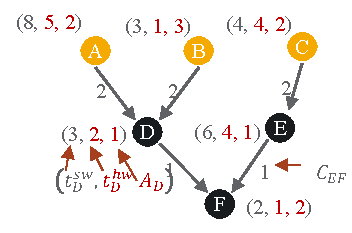
\includegraphics[width=0.52\linewidth]{Figures/methods/demosoftmakespan.pdf}
\caption{Illustrative 6-node fork-join task graph used to explain the differentiable soft scheduler. The accompanying numerical example uses demo values for exposition. Each node is annotated with $(t_i^{sw}, t_i^{hw}, A_i)$, and each edge label denotes communication cost.}
\label{fig:demosoftmakespanI}
\end{figure}



\subsection{Training Objective}

The overall loss for \diffgnn is defined as:
\begin{equation}
L
=
L_{\mathrm{makespan}}(\vp,\vq^{sw})
+
L_{\mathrm{exec}}(\vp)
+
L_{\mathrm{comm}}(\vp)
+
\lambda L_{\mathrm{area}}(\vp)
+
L_{\mathrm{reg}}(\vp,\vq^{sw}).
\end{equation}

Here, $L_{\mathrm{makespan}}$ captures the differentiable scheduling objective, while $L_{\mathrm{exec}}$ and $L_{\mathrm{comm}}$ correspond to relaxed execution and communication costs, respectively, consistent with the soft scheduling formulation.

\paragraph{\textbf{Execution and communication losses.}}
We directly treat the relaxed execution and communication terms as auxiliary losses:
\begin{equation}
L_{\mathrm{exec}}(\vp) = \widetilde{\mathrm{Exec}}(\vp),
\qquad
L_{\mathrm{comm}}(\vp) = \widetilde{\mathrm{Comm}}(\vp).
\end{equation}
These terms guide the model toward efficient hardware/software assignments by penalizing high execution latency and cross-partition communication.

\paragraph{\textbf{Area constraint.}}
To enforce the hardware budget during training, we replace the hard constraint with a differentiable hinge penalty:
\begin{equation}
L_{\mathrm{area}}(\vp)
=
\left[
\max\!\left(
0,\sum_{i\in\gV} p_i A_i - A_{\max}
\right)
\right]^2.
\end{equation}
This penalty activates only when the predicted hardware area exceeds the budget, while preserving the original constrained formulation.

\paragraph{\textbf{Regularization.}}
We further introduce optional regularization to stabilize ordering predictions and encourage nearly discrete assignments:
\begin{equation}
L_{\mathrm{reg}}(\vp,\vq^{sw})
=
\lambda_b L_{\mathrm{binary}}(\vp)
+
\lambda_{\mathrm{perm}} L_{\mathrm{perm}}(\mP^{sw})
+
\lambda_u L_{\mathrm{usage}}(\vp),
\end{equation}
where
\begin{align}
L_{\mathrm{binary}}(\vp)
&=
\frac{1}{n}\sum_{i=1}^n p_i(1-p_i),\\
L_{\mathrm{perm}}(\mP^{sw})
&=
\|\mP^{sw}\mathbf{1}-\mathbf{1}\|_2^2
+
\|(\mP^{sw})^\top\mathbf{1}-\mathbf{1}\|_2^2,\\
L_{\mathrm{usage}}(\vp)
&=
(\tilde{p}-\rho)^2.
\end{align}
Here, $\tilde{p}=\frac{1}{n}\sum_{i=1}^n p_i$ denotes the average hardware usage, and $\rho$ is an optional target utilization ratio.
